% !TeX encoding = UTF-8
% !TeX spellcheck = en_US
% !TeX root = ../MasterThesis_OlivierChurlaud_2016.tex


\documentclass[11pt,oneside,a4paper]{memoir}

% General
\usepackage[utf8]{inputenc}
\usepackage[shorthands=off,english]{babel}
\usepackage{hyperref}
\usepackage{titlesec} 
\usepackage{tabulary}
\usepackage{enumitem}
\setlist{nosep, leftmargin=4em}

% Maths
\usepackage{amsmath}
\usepackage{amsfonts} % caligraphic fonts
\usepackage{amssymb}  % symbols
\usepackage{empheq}   % frame equations
\usepackage{siunitx}  % correct units

% Pictures
\usepackage{graphicx}
\usepackage{caption}
\usepackage{subcaption}
\usepackage{rotating}
\usepackage{epstopdf}
\usepackage{tikz}
\usetikzlibrary{shapes,arrows,positioning}

% Should be loaded last
\usepackage{setspace}
\usepackage[noabbrev]{cleveref}

% Default fixed font does  support bold face

% Custom colors
\usepackage{color}
\definecolor{deepblue}{rgb}{0,0,0.5}
\definecolor{deepred}{rgb}{0.6,0,0}
\definecolor{deepgreen}{rgb}{0,0.5,0}
\definecolor{gray}{rgb}{0.5,0.5,0.4}

\usepackage{listings}
\usepackage{lstautogobble}
\renewcommand{\lstlistingname}{Code example}

% Python style for highlighting
\newcommand\pythonstyle{\lstset{
    language=Python,
    basicstyle=\linespread{1}\footnotesize\ttfamily,
    otherkeywords={self},             % Add keywords here
    keywordstyle=\footnotesize\ttfamily\bfseries\color{deepblue},
    emph={MyClass,__init__},          % Custom highlighting
    emphstyle=\bf\color{deepred},    % Custom highlighting style
    stringstyle=\color{deepgreen},
    frame=tb,                         % Any extra options here
    showstringspaces=false,           % 
    tabsize=4,
    numbers=left,    
    numberstyle=\tiny\color{gray}, 
    breaklines=true,
    autogobble=true,
    commentstyle=\color{gray},           
}}


% Python environment
\lstnewenvironment{python}[1][]
{
\pythonstyle
\lstset{#1}
}
{}

% Python for external files
\newcommand\pythonexternal[2][]{{
\pythonstyle
\lstinputlisting[#1]{#2}}}

\newcommand\cppstyle{\lstset{
    language=C++,
    basicstyle=\ttfamily,
    keywordstyle=\color{deepblue}\ttfamily,
    stringstyle=\color{red}\ttfamily,
    commentstyle=\color{grey}\ttfamily,
    morecomment=[l][\color{magenta}]{\#},
    autogobble=true,
}}

% C++ environment
\lstnewenvironment{c++}[1][]
{
    \cppstyle
    \lstset{#1}
}
{}

% % % % % % % % % % % % % % % % % %
% trick not to release comments   %
  \newif\ifrelease
%	                              %
	%\releasetrue
	\releasefalse
%	                              %
	\ifrelease
	\else
		\usepackage[colorinlistoftodos,textsize=scriptsize]{todonotes}
	\fi
% end of trick                    %
% % % % % % % % % % % % % % % % % %

\renewcommand{\vec}[1]{\underline{#1}}
\newcommand{\mat}[1]{\underline{\underline{#1}}}
\newcommand{\scal}[2]{\langle #1 {\,,\,} #2 \rangle}

\newcommand{\remark}{\paragraph{Remark ---}}
\setsecnumdepth{subsubsection}
%\maxtocdepth{subsection}
\renewcommand{\baselinestretch}{1.5} 
\setlrmarginsandblock{3cm}{2.5cm}{*}
\setulmarginsandblock{3cm}{2.5cm}{*}
\checkandfixthelayout

\def\thetitle{Localization and correction of orbit perturbations in BESSY II storage ring}
\def\thesubject{Master Thesis}
\def\theauthor{Olivier Churlaud}
\def\theauthorinfo{Matriculation number: 366\,964}
\author{\theauthor}
\title{\thetitle}

\hypersetup{
    unicode=true,
    pdftitle={\thetitle},
    pdfauthor={\theauthor},
    pdfsubject={\thesubject},
    colorlinks=true,       % false: boxed links; true: colored links
    linkcolor=teal,       % color of internal links (change box color with linkbordercolor)
    citecolor=olive,
    filecolor=red,
    urlcolor=blue
}

\begin{document}

\frontmatter
\cleardoublepage
\thispagestyle{empty}

% !TeX encoding = UTF-8
% !TeX spellcheck = en_US
% !TeX root = ../MasterThesis_OlivierChurlaud_2016.tex

\begin{titlingpage}
    \noindent
    \renewcommand\arraystretch{0}
    \begin{tabulary}{\linewidth}{l r}
        \begin{minipage}{.45\linewidth}
            \includegraphics[height=70pt]{img/hzb_logo_schwarz}
        \end{minipage}
        &
        \begin{minipage}{.45\linewidth}
            \flushright
            \includegraphics[height=50pt]{img/TU_logo_schwarz}
        \end{minipage}
        \\
        \begin{minipage}[t]{.45\linewidth}
            \begin{SingleSpace}
                \scriptsize
                Helmholz-Zentrum Berlin für Materialien und Energie \\
                Light source BESSY~II  \\
                Department Operation Accelerator (NP-ABS)
            \end{SingleSpace}
        \end{minipage}
        &
        \begin{minipage}[t]{.45\linewidth}
            \begin{SingleSpace}
                \scriptsize
                \flushright
                Technische Universität Berlin \\
                Fakultät IV -- Elektrotechnik und Informatik  \\
                Institut für Energie- und Automatisierungstechnik \\
                Fachgebiet Regelungssysteme  \\
                Prof. Dr.-Ing. Jörg Raisch
            \end{SingleSpace}
        \end{minipage}
    \end{tabulary}

	\vfill

	\begin{center}
	\LARGE \textsc{\thesubject}
	\end{center}

	~

	\begin{Spacing}{3}
		\centering\textsc{\huge\thetitle}
	\end{Spacing}

	\vfill

	\centering
	Submitted by


	\theauthor  ~-- \theauthorinfo

	~

	In partial fulfillment of the requirements for \\ the Degree of Master of Science in Electrical Engineering

	~


	\today

	\vfill


	Supervisors

	~

	\setlength{\tabcolsep}{15pt}
    \renewcommand\arraystretch{.7}
	\begin{tabular}{l l}
		TU Berlin
		&Prof. Dr.-Ing. Jörg Raisch \\
	    ~ & ~\\
			Helmholtz-Zentrum Berlin
		& Prof. Dr. Andreas Jankowiak \\
		~ & Dr. Andreas Schälicke
	\end{tabular}
\end{titlingpage}


\cleardoublepage
\begin{abstract}
       ......
\end{abstract}
\vfill

\cleardoublepage
\tableofcontents*
\listoffigures*

\mainmatter

% !TeX encoding = UTF-8
% !TeX spellcheck = en_US
% !TeX root = ../MasterThesis_OlivierChurlaud_2016.tex

\chapter{Introduction}
\label{sec:background}

\section{BESSY II -- General presentation}
BESSY II (\textbf{B}erliner \textbf{E}lektronen \textbf{S}peicherring-Gesellschaft für \textbf{Sy}n\-chro\-tron\-strahlung m.b.H.) is Berlin's electron storage ring, aimed at producing high energy light ray by synchrotron radiation. It emits extremely brilliant photons pulse ranging from Terahertz to hard X rays, with an emphasis on the soft X-ray range ~\cite{web:bessy_homepage}.

Scientific projects can freely apply for beam time at an experimental station, where they are able to adjust the wavelength, polarization and photon energy. More than 2000 scientists are using BESSY II equipment every year.

The storage ring has a circumference of \SI{240}{\meter} and provides around 50 beamlines (paths of light rays between the storage ring and experimentation stations). The electrons are accelerated to an energy up to \SI{1.7}{\giga\electronvolt}.

BESSY II was inaugurated in 1998 to let scientists study material structures and processes. Since 2009 it is a facility of the \textit{Helmholtz-Zentrum Berlin für Materialien und Energie} (HZB)

Additionally to the guest scientists, operators and researchers ensure the good functioning of the whole facility and work on refining the quality and the stability of the light rays.

\section{BESSY II -- General functioning}
In the BESSY II  accelerator, particles are circularly accelerated, all of them turning in the same direction. The goal is to produce light, instead of collisions.

The way BESSY II functions is based on the synchrotron radiation phenomenon: any accelerated particle emits radiations (in the form of photons). It can be shown~\cite{book:wille} that the radiated power in circular acceleration can be given as
\begin{equation}
P_s = \frac{e^2 c}{6 \pi \varepsilon_0}\frac{1}{(m_0 c^2)^4}\frac{E^4}{R^2}.
\end{equation}
where $c$ is the speed of light, $m_0$ the rest mass (independent of the velocity) of the particle, $e$ its charge, $E$ its energy, $R$ the bending radius and $\varepsilon_0$ the  vacuum permittivity.

Considering their low mass, electrons are very good candidates to produce high energy radiation (in comparison, accelerated protons would provide $10^{13}$ less radiation than electrons), and are therefore used in BESSY~II.

\begin{figure}
    \centering
    \includegraphics[width=0.8\textwidth]{img/bessy_acc_chain_web.jpg}
    \caption[BESSY~II -- Accelerator chain]{\label{fig:bessy_acc_web_simple} BESSY~II -- Accelerator chain (Source:~\cite{web:bessy_homepage})}
\end{figure}

\begin{sidewaysfigure}
    \centering
    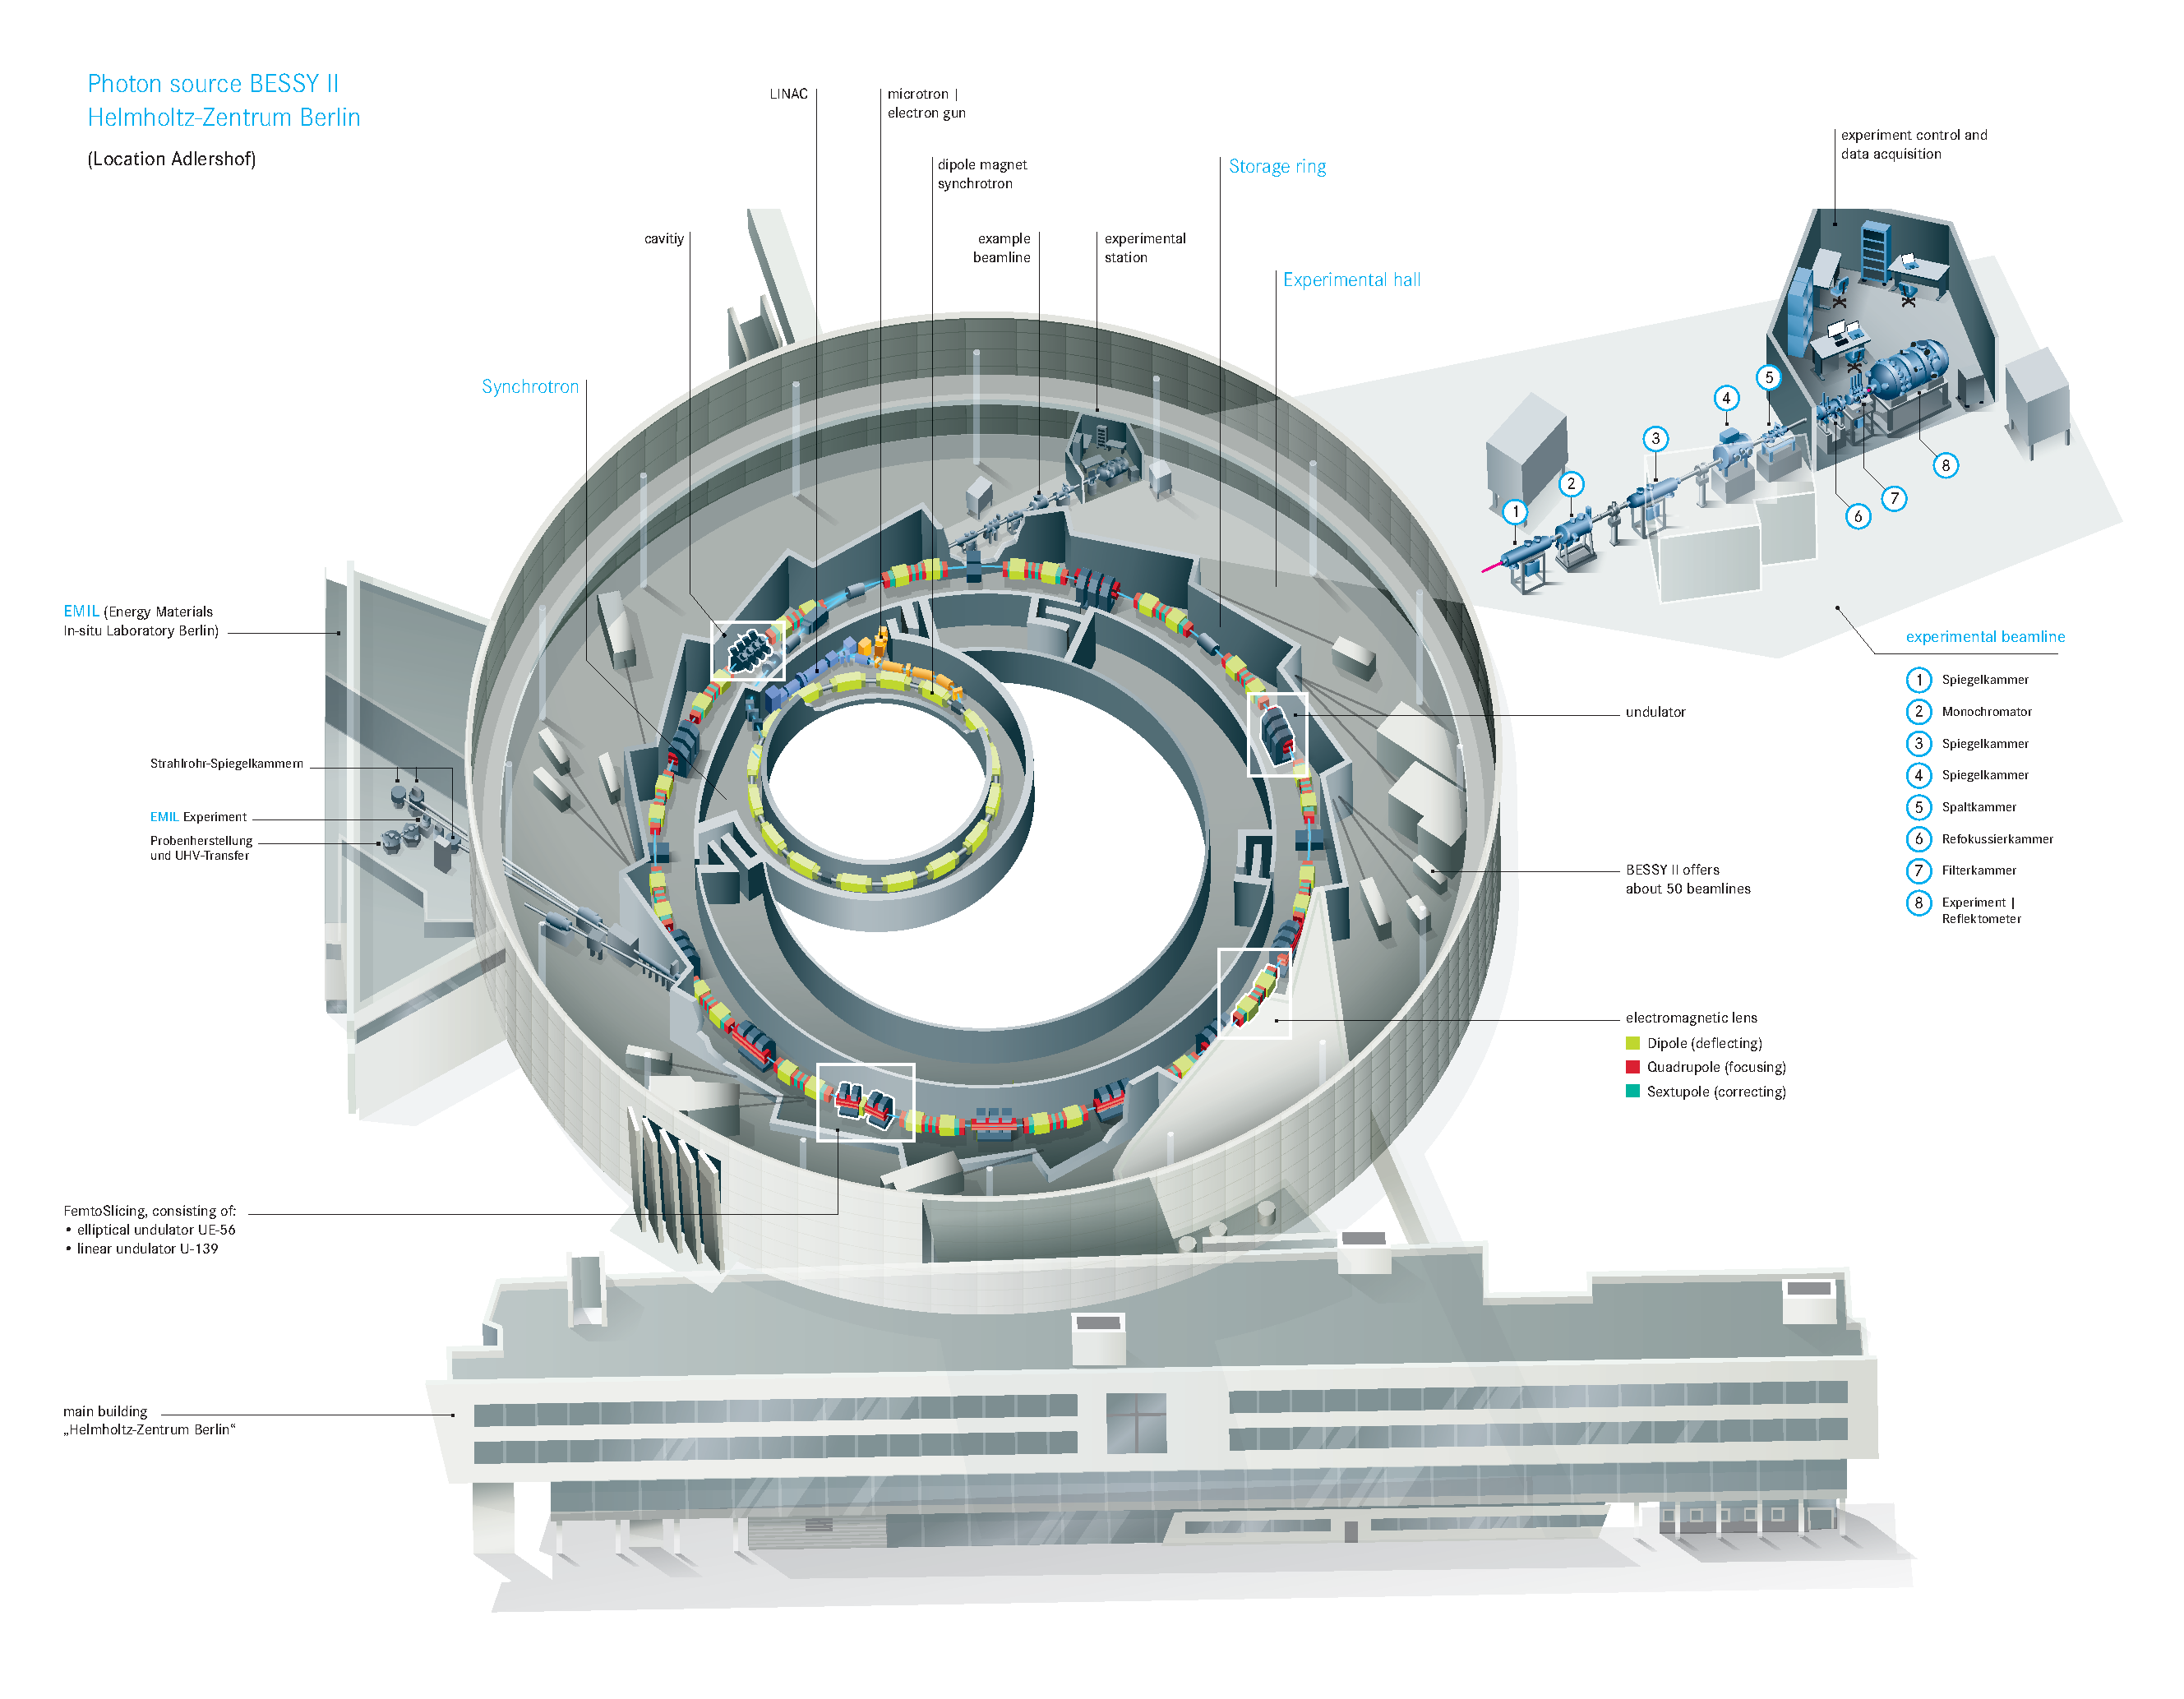
\includegraphics[width=0.9\textwidth,height=1\textheight,keepaspectratio]{img/bessy_acc_web.pdf}
    \caption[BESSY~II facility]{\label{fig:bessy_acc_web} BESSY~II facility (Source:~\cite{web:bessy_homepage})}
\end{sidewaysfigure}

In order to reach an energy of \SI{1.7}{\giga\electronvolt}, the electrons undergo several chained accelerations (see \cref{fig:bessy_acc_web}), namely:
\begin{enumerate}
    \item DC electrons are provided by an electron gun at an energy of \SI{90}{\kilo\electronvolt},
    \item a LINAC (\textbf{lin}ear \textbf{ac}celerator) increase the energy to \SI{50}{\mega\electronvolt},
    \item the booster (a fast rumping synchrotron) accelerate the particles to their full energy of \SI{1.7}{\giga\electronvolt} in not more than \SI{30}{\milli\second}.
\end{enumerate}

When this energy is reached, the electrons are injected to the storage ring, which ensure that the electrons are kept at the same energy.

Another important property of BESSY~II is that it is operated in \textit{top-up mode}. This means that its current must be constant over time (in this case: \SI{300}{\milli\ampere}). However electrons are likely to collide into each other or with the rest-gas atoms of the vacuum chamber. To achieve the top-up mode and counter the loss of electrons, new injections from the acceleration chain take place approximatively every 2~minutes to repopulate the storage ring.

\section{Motivation}
The most important properties of the synchrotron radiation are its brilliance and brightness, which represent the quality of the beam. The brightness describes the angular divergence of the beam, and the brilliance includes information about its transverse dimension: both are expected to be as small as possible to be in the configuration in which the beam is the most point-like. (See \cref{apx:brightness_brilliance} for the exact definitions).

The main purpose of BESSY~II is to provide a light radiation with high quality brilliance and brightness over time. To achieve this, the light source itself must be very stable and the electron beam very small. The stability of the orbit is required to be well bellow the transverse beam dimensions, which are for BESSY~II storage ring \SI{100}{\micro\meter} in the horizontal direction and \SI{20}{\micro\meter} in the vertical one.

Therefore a significant attention is drawn to the control of the storage ring orbit: the beam diameter must be as small as possible and therefore always well centered in the vacuum chamber. Although the storage ring is designed to achieve this, perturbations or misalignment in the accelerator optics must be corrected. Orbit feedback is used here to correct and stabilize the orbit and to keep it focused.

\section{Summary}
BESSY~II is a powerful light source, with a nominal energy of \SI{1.7}{\giga\electronvolt}, that produces a light of high quality, which is a wide spectrum and high brilliance. In order to keep the quality of these properties, removing perturbation sources or correcting the orbit is needed.

In the following, \cref{sec:acc_physics} will provide the needed accelerator physics backgrounds. \Cref{sec:correction} will treat of correction methods, first introducing a state of the art in the particle accelerator community, and more specially at BESSY~II. Based on this, the improvement conducted during this work will be described. \Cref{sec:control} will discuss how models and simulations where conducted in order to propose better controllers. In \cref{sec:localization}, algorithms conceived and implemented during this thesis to localize perturbation sources will be presented. Finally \cref{sec:conclusion} will provide an overview of the results achieved with this work and some insights on how to go further.

\input{tex/accphysics}
% !TeX encoding = UTF-8
% !TeX spellcheck = en_US
% !TeX root = ../main.tex
\tikzset{
	block/.style = {draw, fill=white, rectangle, minimum height=3em, minimum width=4em},
	gain/.style = {draw, fill=white, isosceles triangle, minimum height=3em, minimum width=2em},
	operator/.style= {draw, fill=white, circle},
	input/.style = {coordinate},
	output/.style= {coordinate},
	pinstyle/.style = {pin edge={to-,thin,black}},
}

\chapter{Orbit correction}
\label{sec:correction}

\section{Motivation}
The accelerators are designed so that the particles follow a given path, which is defined in the case of synchrotrons by the successive bendings involved by the magnets. As the precision of the positioning of the magnets is limited, some errors may destabilize the orbit and increase the dispersion of the particles around the theoretical orbit. In addition, the environment produces perturbations: for instance the 50~Hz of the main power, some not perfectly isolated magnetic sources.

In order not to lose electrons in the walls of the vacuum chamber but also to increase the brightness of the synchrotron radiations (and therefore to have focused electron beams), all these residual misalignment and magnetic field errors must be corrected.



\section{Monitoring and correction instruments}
To be able to correct the orbit or localize perturbations, some tools must be employed.

\subsection{Beam Position Monitors}
The position of the beam in a given direction is monitored with beam position monitors (BPM). 

Several types of BPMs exist, but the important characteristics of the one used at BESSY~II are that they provide a method
\begin{itemize}
	\item which is non invasive (it does not affect the beam or negligibly)
	\item which outputs an electric signal proportional to the distance of the beam from an arbitrary point.
\end{itemize}

This last property means that the measured value must always be subtracted by a reference value.

The raw values output by the BPMs are thus never considered and every orbit position value given (also called BPM value by misuse of language) is always, at position~$s$ and time~$t$
\begin{equation}
\Delta x_\text{BPM}(s,t) = x_\text{BPM}(s,t) - x_\text{BPM,ref}(s)
\end{equation}

\subsection{Correctors}
To correct the orbit, BESSY~II uses dipoles, also called correctors (CM) disposed around the orbit. Each dipole contributes to correcting in a given direction. 

\subsection{Monitor and corrector numbers}
The number of monitors and correctors is quite important. Because the correction method used is based on an inversion problem (see \cref{sec:response_matrix}), it is important to have an over-constrained problem. Else a perfect correction would be reached at monitor positions but unconstrained (and thus potentially arbitrary bad) elsewhere.

Therefore the number of BPMs is chosen quite greater than the number correctors.

In BESSY~II there are 
\begin{itemize}
	\item 128~BPMs, measuring both horizontal ($\text{BPM}_x$) and vertical ($\text{BPM}_x$) direction,
	\item 48~CMs for the horizontal direction ($\text{CM}_x$) and 64 for the vertical one ($\text{CM}_y$).
\end{itemize}

\section{Some documented methods}
Several global corrections methods are well documented in the literature. Local orbit bumps (presented in \cref{sec:orbit_bump}) allow local correction and are used to change the path of the orbit (during the injection time for example). The most common ones are the best corrector method and the response matrix method (see \cref{sec:most_effective_corr,sec:response_matrix}), as they provide a global correction, over the whole orbit. 

\subsection{Local orbit bumps}
\label{sec:orbit_bump}
Using local orbit bumps is a basic method that gives total control on the orbit local modification to the operator.

\subsubsection{Principle}
Adding a simple dipole on the path of a particle will focus or defocus it. As the particles must eventually return to the planned orbit, a series of dipoles can be set one after the other to design an arbitrary path. \Cref{fig:local_bump} shows a minimal example, where the black points represent the magnets. 
\begin{figure}
	\centering
	\begin{tikzpicture}[auto, node distance=1.2,>=latex']
	%\draw[help lines, yellow] (-1,-4)grid(15,3);
	% We start by placing the blocks
	\coordinate [] (lleft) {};
	\node [draw, circle, fill=black, right=2 of lleft] (leftm) {};
	\node [draw, circle, fill=black, above right=2 and 2.5 of leftm] (topm) {};
	\node [draw, circle, fill=black, right=5 of leftm] (rightm) {};
	\coordinate [right=2 of rightm] (rright) {};
	% Once the nodes are placed, connecting them is easy. 
	\draw [-] (lleft) -- node {}(leftm);
	\draw [-] (leftm) -- node {}(topm);
	\draw [-] (topm) -- node {}(rightm);
	\draw [-] (rightm) -- node {}(rright);
	\end{tikzpicture}
	\caption{\label{fig:local_bump}Local bump with 3 magnets}
\end{figure}
\todo[inline]{see Wille p127 and p286}


\subsubsection{In practice}
This solution is used for instance to shift a part of the orbit during particle injections, in order to prevent collisions. This can also be used to counter a known localized perturbation which source cannot be removed.

It is indeed very efficient to locally shift the orbit. However it cannot be used for correction, as it modify the path of the orbit itself, introducing maybe other perturbations.

\subsection{Most effective corrector method}
\label{sec:most_effective_corr}
This method is based on the fact that orbit shifts are often caused by strong localized disturbances. Its goal is to correct particularly each disturbance.

\subsubsection{Principle}
Given a distorted orbit, the optimal gain for each corrector is calculated by a mean square error algorithm (see \cref{eq:gain_bestcorr} and \cite{book:wille}). The corrector which provides the best correction is selected: it is the most effective corrector.

Let's assume that the $i$th corrector, at position $s_i$, has the optical parameters $\beta_i$, $\alpha_i$ and $\Psi_i$, and that $m$ monitors are set around the orbit with parameters $\beta_j$, $\alpha_j$ and $\Psi_j$, and read a displacement $u_j$ from the reference orbit ($1 \leq j \leq m$).

The strength $\kappa_i$ of the field at the position $s_i$ is obtained minimizing the function
\begin{equation}
	\label{eq:gain_bestcorr}
    f_i(\kappa_i) = \sum\limits_{j=1}^{m} (u_j-x_{ij}(\kappa_i))^2 
                  = \sum\limits_{j=1}^{m} (u_j- \kappa_i h_{ij})^2
\end{equation}

with, if $\Delta \Psi_{ij} := \Psi_j-\Psi_i$,

\begin{align}
    \label{eq:hij}
    x_{ij}(\kappa_i) &= \kappa_i h_{ij} \nonumber\\
                     &= \kappa_i \frac{\sqrt{\beta_i \beta_j}}{2}
                         \left[
                             \frac{\cos(\Delta \Psi_{ij}) - 2\alpha_i \sin(\Delta\Psi_{ij})}
                                  {\tan (\pi Q)} + \sin (\Delta\Psi_{ij})
                         \right].
\end{align}

It follows that 
\begin{equation}
    \kappa_i = \frac{\sum\limits_{j=1}^m u_j h_{ij}}{\sum\limits_{j=1}^m h_{ij}^2}
\end{equation}

The $i$th corrector is attributed the gain $-\kappa_i$ to compensate the field.

\subsubsection{Iterative version}
When the most effective corrector is found, the process is reiterated on the corrected orbit with the remaining correctors. By doing this until all corrector are used (or that adding a correction does not improve the orbit) a comprehensive correction is reached.

\subsubsection{Practical issue}
The problem of this method is that each corrector must be tested once, and this for each iteration: the initialization of the correction is long and is then fixed. Moreover, the correction is less efficient than the other ones presented here~\cite{book:wille}.

\subsection{Inversion of the response matrix}
\label{sec:response_matrix}
This section is mainly based on~\cite{book:wille}, \cite{art:decker-1991} and \cite{art:plouviez-1999}.

\subsubsection{Inverse problem}
This correction is based on solving the following inverse problem: the expected orbit being known, how to set the correctors in order to achieve it? To solve it, the response matrix $\mat{S}$ is introduced.

The response matrix $\mat{S}$ is defined by the equation $\vec{X} = \mat{S}\, \vec{\Theta}$ where $\vec{\Theta}$ is the \emph{kick vector} (i.e. the vector of strength of the field generated by each corrector) and $\vec{X}$ the vector of \emph{orbit change}. If the accelerator has $M$ monitors and $N$ correctors, then $\mat{S}$ is a $M \times N$ matrix. $\mat{S}$ is often termed \emph{forward} or \emph{observation matrix} because it describes the effects of a given phenomenon. Indeed, each coefficient $S_{ij}$ of the matrix is the orbit change at the position $s_i$ (of the $i$th monitor), for a kick of unity 1 at the position $s_j$ (of the $j$th corrector).

Inversing the response matrix will provide the correction to apply. Since it's very common to have more monitors than correctors, the matrix is not square. A \emph{singular value decomposition} (SVD) is used on the matrix to provide a pseudo-inversion $\mat{S}^*$ of $\mat{S}$.

Using the SVD also allows to use only the most significant singular values in the correction. This prevents to over-correct the orbit, by not considering less significant values that can result of noise in the monitors during the measure, or numerical artifacts for instance.

The correction can then be performed
\begin{equation}
\vec{\Theta} = \mat{S}^* \vec{X}.
\end{equation}

\subsubsection{Acquisition of the response matrix}
Before solving the inverse problem, the response matrix must first be determined. This can be achieved in two different ways: by describing the magnet structure and explicitly calculating the matrix or by acquiring it in an experimental way.

\paragraph{Calculation of the response matrix}
The matrix can be theoretically calculated by using the accelerator model and physics. This was already used in \cref{sec:most_effective_corr} and using the same calculations leads to setting, for the $i$th monitor and $j$th corrector,
\begin{equation}
S_{ij} = h_{ij}
\end{equation}
with $h_{ij}$ as defined in \cref{eq:hij}.

The main flaw of this method is that it is only a model which hence may not exactly represent the reality. Some misalignments of magnets or external magnetic perturbations would not be taken in account. It's however a good first approach.

\paragraph{Experimental acquisition of the response matrix}
A more common and precise way of constructing the response matrix is empirical: it suffices to give a unitary value to a corrector and to read the monitors to obtain a column $\mat{S}$. Doing so for each corrector provides the whole matrix.


\section{State of the art at BESSY II}
\label{sec:correction_state_of_art}
\subsection{The correction}
BESSY II currently uses a Fast Orbit Feedback (FOFB) which is based on a PID correction (proportional response with gain $K_p$, integral response with gain $K_i$ and derivative response with gain $K_d$) and the response matrix inversion. The full process goes as presented in \cref{fig:block_correction}.

\begin{figure}
    \centering
    \begin{tikzpicture}[auto, node distance=1.2,>=latex']
    %\draw[help lines, yellow] (-1,-4)grid(15,3);
        % We start by placing the blocks
        \node [operator] (sum) {$+$};
        \node [input, above=2 of sum.center] (xref) {};
        \node [operator, right=of sum] (prod) {$\times$};
        \node [input, above=2 of prod.center] (invS) {};
        \node [gain, right=0.7 of prod] (gain) {$\vec{W}$};
        \node [block, right=of gain] (PID) {~PID~~};
        \node [input, above=2 of PID.center] (pidcoef) {};
        \node [operator, right= of PID] (sum2) {$+$};
        \node [block, above right= 0.8 and 0.65 of sum2.center] (delay) {Delay T};
        \coordinate [right=3 of sum2.center] (straight) {};
        \node [draw, ellipse, minimum height=1.7cm, minimum width=5.5cm, below=1 of straight] (ring) {Storage Ring};
        \node [draw, ellipse, line width=1pt, dotted, minimum height=.5cm, minimum width=.8cm, above=-.25 of ring.north, label=above right:\footnotesize Correctors] () {};
        \node [draw, ellipse, line width=1pt, dotted, minimum height=.5cm, minimum width=.8cm, above=-.25 of ring.west, label=above left:\footnotesize BPMs] (BPM) {};
        \coordinate [left=1 of sum.center](leftback) {};
        
        % Once the nodes are placed, connecting them is easy. 
        \draw [->] (xref)     -- node [pos=0.85, left]{$-$} node {$\vec{X}_\text{ref}$}(sum);
        \draw [->] (sum)      -- node {$\Delta\vec{X}$} (prod);
        \draw [->] (invS)     -- node {$\mat{S}^*$}        (prod);
        \draw [->] (prod)     -- node {}             (gain);              
        \draw [->] (gain)     -- node {$\Delta\vec{\Theta}_\text{t}$}             (PID);
        \draw [->] (PID)      -- node {$\Delta\vec{\Theta}$} node[pos=0.80, below] {$-$}      (sum2);
        \draw [->] (pidcoef)  -- node[pos=0.70, above, fill=white] {PID coeff.} (PID);
        \draw [-]  (sum2)     -- node {}  (straight);
        \draw [->] (straight) |- node[pos=0, right] {$\vec{\Theta}_{(n)}$} (delay);
        \draw [->] (delay)    -| node[above] {$\vec{\Theta}_{(n-1)}$} (sum2);
        \draw [->] (straight) -- node[pos=0.80] {}  (ring);


        \draw [-]  (ring)     -| node {}             (leftback);
        \draw [->] (leftback) |- node[pos=0.5] {$\vec{X} $}  (sum.west);
\end{tikzpicture}
    \caption{\label{fig:block_correction}The correction process}
\end{figure}

The control value at correction cycle $n$ is the differential orbit 
\begin{equation}
 \Delta \vec{X}(n) := \vec{X}(n)-\vec{X}_\text{ref}
\end{equation}
which is expected to be 0. The correction provided by the weighted response matrix is then processed
\begin{equation}
\Delta \vec{\Theta}_\text{t}(n) :=  \left[ \mat{S}^{-1} \cdot \Delta \vec{X}(n) \right] \odot \vec{W}
\end{equation}
(with $\odot$ the point-wise multiplication and $\vec{W}$ the vector of weights) and modulated by the PID correction. The ideal PID has the form
\begin{equation}
H_{PID}(s) = K_p + \frac{K_i}{s} + K_d \cdot s 
\end{equation}
or, with the z transform (calculated with Euler's method),
\begin{equation}
H_{PID}(z) = K_p + \frac{K_i}{1-z} + K_d \cdot (1-z)
\end{equation}
which yields
\begin{equation}
\Delta \vec{\Theta}(n) =  K_p \cdot \Delta \vec{\Theta}_\text{t}(n) + K_i \cdot \sum\limits_{k=0}^{n-1}\Delta \vec{\Theta}_\text{t}(k) + K_d \cdot \left[\Delta \vec{\Theta}_\text{t}(n) - \Delta \vec{\Theta}_\text{t}(n-1)\right].
\end{equation}

The real correction is eventually the accumulation of all corrections
\begin{equation}
\vec{\Theta}(n) = \vec{\Theta}(n-1) - \Delta \vec{\Theta}(n).
\end{equation}

For stability reasons, the PID was always implemented as a proportional corrector ($K_i$ ad $K_d$ being zero) which was behaving as a proportional integrator (PI) because of the last accumulation. \todo{implemented in the future? or see section XXX}

\remark The PID gains is not exactly as presented here: to prevent a too violent correction that might destabilize the current in the ring, the proportional gain is increased every correction cycle by 1\% until it reaches its nominal value.

\subsection{Technical overview}

The correction is naturally automatized. Because the read/write actions should be really fast, a specific infrastructure was designed. This is represented on \cref{fig:cbox_mbox}. 

\begin{figure}[!h]
    \centering
    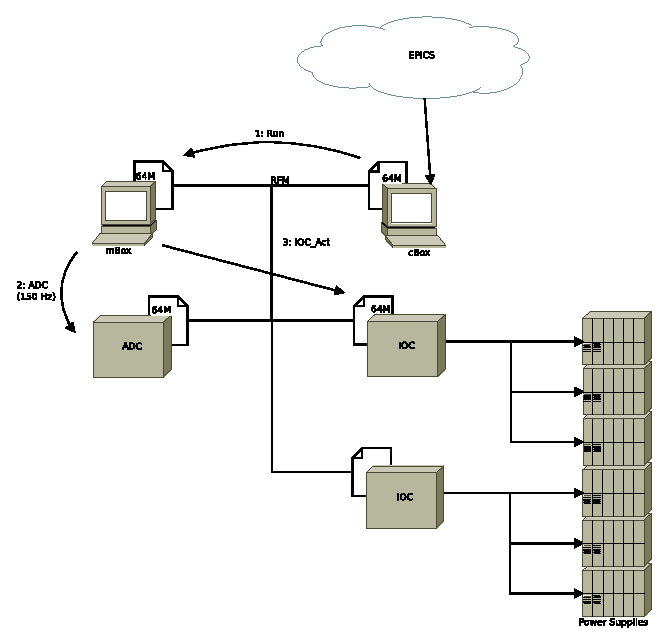
\includegraphics[width=.85\linewidth]{img/mBox_cBox}
    \caption{\label{fig:cbox_mbox}cBox and mBox: the correction infrastructure in BESSY II}
\end{figure}

All elements are connected to a reflective memory (RFM), which provides a high speed and low latency interface. This memory space is split in specified divisions to prevent data collisions: one part contains the configuration, a second the orbit values and the last one the correction values.

The following actors are playing a role in the process:
\begin{itemize}
    \item the \textbf{cBox} which controls (= \textit{c}) the correction. It defines when to read the values of the BPMs and when to write the new correction values, it provides initializations values. The operators are communicating with this process to configure the correction.
    \item the \textbf{mBox} which does the math (= \textit{m}) of the correction. When allowed by the cBox, it reads the BPMs values, do the maths to define the new correction values (multiplication with the response matrix, PID correction) and write them to the communication bus. This process also publish the values it reads and writes so that client programs can subscribe to this data stream and reuse the values internally.
    \item the \textbf{Input-Output Controllers (IOCs)} write the correction values to the power supplies commands when they are available.
    \item the \textbf{power supplies (PS)} provide a given power to the corrector magnets.
\end{itemize}

After having received the authorization to run from the cBox, the mBox process starts. It first do its full initialization, which only happens on start (the response matrix, the reference orbit, the PID parameters, etc. cannot change while the mBox process is running), and starts the ADC (Analog-to-Digital Converter). From this time, they will write new orbit values to the RFM at a rate of \SI{150}{\hertz}.

The mBox waits for the ADC interruption to read the new orbit data from the RFM. The correction is then calculated (in Amperes) and the values are converted in a format easily transmissible (basically unsigned integers). This data is written back to RFM and an interruption is sent to inform the other elements that the new values are available. This is read by the IOCs that relay to the power supplies alimenting the corrector magnets. 

This defines a real time process, repeated at the frequency of \SI{150}{\hertz}.

The duration of each step is as following:\todo{TIMES}
\begin{enumerate}
\item orbit value acquisition: \SI{00}{\milli\second}
\item correction computation: \SI{00}{\milli\second}
\end{enumerate}

\section{Improvement of the correction for harmonic perturbations}
The correction presented until now only provides a temporal correction. It has no possibility to correct a specific harmonic or to perform in the spectral domain.

A simple extension of this method is to analyze a given harmonic of the orbit, and consider the Fourier coefficient of each monitor as the complex amplitude of the orbit
\begin{equation}
	\forall f \in \mathbb{R}, \qquad c_f = \frac{2}{T} \int_0^T x(t) e^{-j 2 \pi f t} dt
\end{equation}
or, in the digital domain,
\begin{equation}
\forall f \in \left[0, \frac{Fs}{2}\right], \qquad c_f = \frac{2}{N} \sum\limits_{k=0}^{N-1} x(k) e^{-j 2 \pi f \frac{k}{F_s}}
\end{equation}
where $F_s$ is the sampling frequency, $f = \frac{1}{T}$ the frequency of interest and N the number of samples.

Because of the digitalization, $f$ must be a multiple of $\frac{F_s}{N}$, which can be a problem here. The complex amplitude is therefore used as initial value in a least-square-error fit-curve algorithm that will provide a hopefully more precise amplitude if the frequency of interest did met the precedent condition.

This provides an complex orbit $\Delta\vec{X}_f$ for the harmonic $f$. From there the corrector values can be calculated with the traditional method
\begin{equation}
\Delta\vec{\Theta}_f = \mat{S}^{1}\, \Delta\vec{X}_f   \in \mathbb{C}.
\end{equation}

To apply the correction, an oscillation must finally be generated with the obtained parameters. This is, for the $i$th corrector
\begin{equation}\label{eq:th_dyn_corr}
\forall t \in  \mathbb{R}, \qquad y(t) = \left| \Delta\vec{\Theta}_f(i) \right| \cdot \cos\left(2 \pi f t - \arg\left(\Delta\vec{\Theta}_f(i)\right)\right).
\end{equation}

The main problem with this method is that the generated signal phase must be synchronized with the time the correction parameters were measured. This was possible only for perturbations for which the source was already known and could be used as reference signal.

\subsection{Example of the 10 Hz perturbation}
The \SI{10}{\hertz} perturbation has a well known source which is the booster power supply (pre-accelerator). This perturbation has such a great impact on the orbit spectrum and could be used as a validation case.

A coil was used to measure the field generated by a magnet powered by the same source as the booster. It provides a \SI{10}{\hertz} reference which is synchronized with the perturbation.

The orbit and the reference signal were measured during the exact same time. Both were analyzed with the method presented above. Instead of using \cref{eq:th_dyn_corr}, the reference signal was used and its phase and amplitude where changed for each corrector with the help of a finite impulse response (FIR) filter. Because the sampling frequency is \SI{150}{\hertz}, a FIR with 15 taps for the $i$th corrector can be designed as follow
\begin{equation}
	h_i(n) = \frac{\left| \Delta\vec{\Theta}_f(i) \right|}{\left|A_{10}\right|} \cdot \cos\left(2\pi\cdot \frac{10}{150} n - \left[\arg\left(\Delta\vec{\Theta}_f(i)\right) - \phi_{10}\right] \right),\quad n \in 0..14
\end{equation}
where $A_{10}$ and $\phi_{10}$ are respectively the amplitude and the phase of the reference signal.

This can then be applied to the reference signal $x_{10}$: for the $i$th corrector, the dynamic correction is
\begin{equation}
y[n] = \sum\limits_{k=0}^{14} h[k] x_{10}[n-k]
\end{equation}

\section{System and correction simulation}
One difficulty in improving the current correction process is that machine time is expensive: tests cannot be done very often. A wrong correction can indeed destabilize the orbit or worse, lose the electrons in the vacuum chamber walls, and thus it cannot be tested when the storage ring is on service or other scientists do experiments or measurements for their own research. However, has presented previously, the process is complex and it must be sure that every actors will play correctly in an improved process. Simulating the whole environment is expected to mitigate this.

\subsection{System identification}
The first step in the model is to represent the storage ring. This could be done analytically, by writing the magnet equations and deriving the full differential equations that bind the correction to orbit displacement. However, it would take a full master thesis to realize a good model, as there are very different types of components all around the orbit, with some non linear behavior.

Instead a system identification is conducted. A brief theoretical explanation will be followed by the actual results.

\subsubsection{Theoretical background}
\todo{Organize it so that it looks like control theory}
A linear time invariant system (LTI) is described by its transfer function
\begin{equation}
	G(s) = \frac{Y(s)}{U(s)}
\end{equation}
where a $Y(s)$ is the Laplace transform of the system output and $U(s)$ the Laplace transform of its input.

\subsubsection{Results}
\todo[inline]{TODO}
\subsection{Simulation model}

\begin{sidewaysfigure}
    \centering
    \begin{tikzpicture}[auto, node distance=1,>=latex']
    %\draw[help lines, yellow] (-1,-4)grid(15,3);
    % We start by placing the blocks
    \node [input] (xref) {};
    \node [operator, right=1.5 of xref] (sum) {$+$};
    \node [block, right=of sum] (correct) {Correction};
    \node [block, right=of correct] (DAC) {$\uparrow$};
    \node [block, right=of DAC] (delay) {Delay T};
    \node [operator, right=of delay] (sumperturb) {$+$};
    \node [input, above=of sumperturb] (perturb) {};
    \node [block, right=of sumperturb] (Hring) {$\text{H}_\text{ring}$};
    \node [block, below=of delay] (ADC2) {$\downarrow$ \SI{150}{\hertz}};
    \coordinate [right= of Hring] (connectout) {};
    \node [input, right= of connectout] (out) {};
    
    % Once the nodes are placed, connecting them is easy. 
    \draw [->] (xref)     	-- node [pos=0.2] {$\vec{X}_\text{ref}$}
							   node [pos=0.85, below]{$-$}  (sum);
    \draw [->] (sum)      	-- node {$\Delta\vec{X}$}    	(correct);
    \draw [->] (correct)  	-- node {}                   	(DAC);
    \draw [->] (DAC)      	-- node {}                   	(delay);
    \draw [->] (delay)    	-- node[above] {}            	(sumperturb);
    \draw [->] (perturb)  	-- node {$d$}               	(sumperturb);
    \draw [->] (sumperturb) -- node {}                		(Hring);
    \draw [-]  (Hring)    	-- node {}                 		(connectout);
    \draw [->] (connectout) -- node {}                 		(out);
    \draw [->] (connectout) |- node {}                 		(ADC2);
	\draw [->] (ADC2)     	-| node[pos=0.5] {$\vec{X}$}	(sum.south);
    \end{tikzpicture}
    \caption{\label{fig:model_simul}The full model}
\end{sidewaysfigure}
\todo[inline]{TODO}

\subsection{Simulation results}
\todo[inline]{TODO}
% !TeX encoding = UTF-8
% !TeX spellcheck = en_US
% !TeX root = ../MasterThesis_OlivierChurlaud_2016.tex

\chapter{Localization of orbit perturbations}
\label{sec:localization}

 A correction, as adapted as it can be, will never be perfect. Instead of dealing with the effects of the perturbation, its sources can first be investigated. When all possible sources are found and removed or isolated, a correction algorithm can be applied to the remaining perturbations, which will hopefully yield to better results.

 If no source is really obvious (e.g. a non-isolated transformer, the \SI{50}{\hertz} perturbation of the main power), the orbit itself can give some hints to localize it. One local perturbation affects indeed the whole revolution. It results in an oscillation across the orbit which, because of the closed orbit property, will brutally change its angle at the position of the source  brutally changes its angle (see \cref{fig:kick}). This position is termed \textit{kick}.

\begin{figure}[!h]
	\centering
	\includegraphics[width=.9\linewidth]{img/kick}
	\caption{\label{fig:kick}Example of kick in the orbit}
\end{figure}

Two types of perturbations will be described in this section:
\begin{itemize}
	\item static perturbations, which can be  for instance a malfunctioning magnet,
	\item harmonic perturbations, i.e. a perturbation at a given frequency, which can be for instance the \SI{50}{Hz} magnetic field of the main power or the \SI{10}{Hz} field due to a bad isolated power supply.
\end{itemize}

\section{Static perturbation}
\label{sec:loc_static}

\subsection{Theoretical setting of the problem}
The problem is described with the betatron phase variable
\begin{equation}
\Psi = \int\limits_{0}^s \frac{d\sigma}{\beta(\sigma)}.
\end{equation}

The spatial variable $s$ is only used to have a connection between the result and the actual ring. The explanation will be led in the horizontal plane (with the $x$ variable), but is also valid in the vertical one ($y$).

Let one kick be at a given phase $\Psi = \hat{\Psi}$. The orbit is modified and oscillates with a constant period of \SI{2 \pi}{\radian}. Because there is \emph{only one} kick and according to the closed orbit condition, the oscillation after the kick will be stable for one revolution. Furthermore, the orbit must be continuous on all points, thus at the kick position too. This is illustrated in \cref{fig:kick}.

Two revolutions are considered, in order to be sure to find one full revolution without kick. Let $\Psi_\mathrm{ext} \in [0, 4 \pi Q]$ be this new phase (\textit{ext} for extended). The phase $\hat\Psi$ where the kick happens is the one so that
\begin{equation}
\exists (b, c) \in \mathbb{R}^2:
\forall \Psi \in [\hat\Psi, \hat\Psi + 2 \pi Q], \quad
x(\Psi) = b \cos(\Psi + c)
\end{equation}
where Q is the tune of the orbit (see \cref{eq:tune}).

This problem has 3 unknowns which should be determined: $\hat\Psi, b, c$.

\subsection{Practical setting}
In order to know the position of the orbit, BPMs are used.

Only $m$ BPMs are distributed around the orbit. The previous variable can thus be described in a vectorial form
\begin{align}
\begin{cases}
\vec{\Psi} = [\Psi_0, \Psi_1, ..., \Psi_{m-1}] \\
\vec{x} = [x_0, x_1, ..., x_{m-1}]
\end{cases} \quad \mathrm{and} \quad
\begin{cases}
\vec{\Psi}_\mathrm{ext} = [\vec{\Psi}, \vec{\Psi}+2\pi Q ]\\
\vec{x}_\mathrm{ext} = [\vec{x}, \vec{x}]
\end{cases}
\end{align}

\subsection{Solving the problem}

The problem is solved in two steps: first the sine that fits at best the orbit is determined, and second the position of the kick verifying the closed orbit condition (or continuity condition) is found.

An algorithm is designed to find a sine over a revolution, beginning at each BPM and keep the one that fits at best:
\begin{align}
\forall~k \in \, &[0,m-1], \nonumber \\
&\begin{cases}
\vec{\Psi}^k = [\vec{\Psi}_\mathrm{ext}(k), \vec{\Psi}_\mathrm{ext}(k+1), \cdots,  \vec{\Psi}_\mathrm{ext}(k+m-1)]\\
\vec{x}^k = [\vec{x}_\mathrm{ext}(k), \vec{x}_\mathrm{ext}(k+1), \cdots,  \vec{x}_\mathrm{ext}(k+m-1)]\\
\tilde{\vec{x}} = \mathtt{fit\_sine}(\vec{x}^k, \vec{\Psi}^k)
\end{cases}
\end{align}

It is then defined
\begin{equation}
k_0 = \underset{k \in [0, m-1]}{\textrm{argmin}}\{||\tilde{\vec{x}}-\vec{x}^k||_2\}
\end{equation}

If there where no noise in the signal, and if the number $m$ of BPMs was infinite, then the kick would be exactly at $\Psi_{k_0}$. However in the real case (with noise), it can only be said that the kick is around $\Psi_{k_0}$, and the closest sine is $\tilde{x}(\Psi) = b \sin(\Psi + c)$.

To find the exact position of the kick, the property of closed orbit is used: the orbit must be continuous also at the kick phase, which means that $\hat{\Psi}$ is the solution of
\begin{align}
b \sin(\Psi + c) &= b\sin(\Psi+c+2 \pi Q),\\
& \mathrm{with}~ \Psi \in [\Psi_{k_0}-A, \Psi_{k_0}+A] , A>0 \nonumber
\end{align}
\begin{align}
&\begin{cases}
\Psi + c &\equiv \Psi + c + 2 \pi Q \pmod{2 \pi} \\
\Psi + c &\equiv \pi - (\Psi + c + 2 \pi Q) \pmod{2 \pi}
\end{cases} \nonumber\\
\iff &\begin{cases}
2 \pi Q &\equiv 0\pmod \pi \qquad\qquad\textit{(Never true)}\\
\Psi &\equiv \left(\frac{1}{2} - Q\right) \pi - c \pmod \pi
\end{cases} \nonumber
\end{align}

The only possible solutions have the form
\begin{equation}
 \Psi \equiv \left(\frac{1}{2} - Q\right) \pi - c \pmod \pi.
\end{equation}
As the kick is the closest solution to $\Psi_{k_0}$, a constant $K$ is searched so that
\begin{align}
&\left(\frac{1}{2} - Q\right) \pi - c + K \pi  \leq \Psi_{k_0} \leq \left(\frac{1}{2} - Q\right) \pi - c + (K+1) \pi \\
\iff  &\left(Q - \frac{1}{2}\right) + \frac{\Psi_{k_0} + c}{\pi}\leq K \leq \left(Q - \frac{1}{2}\right) + \frac{\Psi_{k_0} + c}{\pi} +1 \\
\iff & K = \left\lfloor \left(Q - \frac{1}{2}\right) + \frac{\Psi_{k_0}+c}{\pi} \right\rfloor
\end{align}
and the two remaining possible values are
\begin{equation}
\left\lbrace \left(\frac{1}{2} - Q\right) \pi - c + K \pi , \quad \left(\frac{1}{2} - Q\right) \pi - c + (K+1) \pi\right\rbrace
\end{equation}
the kick being chosen as the closest one from $\Psi_{k_0}$.

\subsection{Finding the good sinusoidal}
Several methods are possible to find the best matching sine, for example by using:
\begin{itemize}
	\item a pseudo-inversion
	\item a scalar-product with a sine (resp. a cosine)
\end{itemize}

\paragraph{Pseudo-inversion}
The problem can be set as a linear equation problem as follow.
\begin{align}
&\forall k \in [0,m-1], \tilde{x}(\Psi_k) = a_1 \cos(\Psi_k) + a_2 \sin(\Psi_k) + a \nonumber \\
%
\implies &
\begin{pmatrix}
1 & \cos(\Psi_0) & \sin(\Psi_0) \\
1 & \cos(\Psi_1) & \sin(\Psi_1) \\
\vdots & \vdots & \vdots \\
1 & \cos(\Psi_{m-1}) & \sin(\Psi_{m-1}) \\
\end{pmatrix}
\begin{pmatrix}
a \\ a_1 \\ a_2
\end{pmatrix}
=
\begin{pmatrix}
x_0 \\ x_2 \\ \vdots \\ x_{m-1}
\end{pmatrix} \nonumber
\\
%
\implies &
\begin{pmatrix}
a \\ a_1 \\ a_2
\end{pmatrix}
=
\mathrm{pseudo\_inv}
\begin{pmatrix}
1 & \cos(\Psi_0) & \sin(\Psi_0) \\
1 & \cos(\Psi_1) & \sin(\Psi_1) \\
\vdots & \vdots & \vdots \\
1 & \cos(\Psi_{m-1}) & \sin(\Psi_{m-1}) \\
\end{pmatrix}
\begin{pmatrix}
x_0 \\ x_2 \\ \vdots \\ x_{m-1}
\end{pmatrix}
\end{align}

The pseudo inverse is calculated in \texttt{Matlab} with
\begin{verbatim}
        a = M\x
\end{verbatim}
and in \texttt{Python} with the least-squares method
\begin{verbatim}
        a = numpy.linalg.lstsq(M, x).
\end{verbatim}

\paragraph{Projection on cosine/sine planes}
Since the orbit is expected to be written as
\begin{equation*}
x(\Psi) = a+ a_1 \cos(\Psi) + a_2 \sin(\Psi)
\end{equation*}
it can also be described as
\begin{equation}
x(\Psi) = \scal{x}{1} + \scal{x}{\cos} \cos(\Psi) + \scal{x}{\sin} \sin(\Psi)
\end{equation}
with $\scal{f}{g}$ being the scalar product for real functions: $\int_T f(t)g(u)dt$.

In the numerical case, the scalar product is approximated by its vectorial counterpart by
\begin{align*}
\scal{\vec{f}}{\vec{g}}: \quad
 &\mathcal{R}^n \times \mathcal{R}^n \longrightarrow \mathcal{R} \\
 & (\vec{f},\vec{g}) \quad\longmapsto \quad \frac{1}{n}\sum\limits_{k=0}^{n-1} f_i g_i
\end{align*}

This however provides less good results, as $\sin(\Psi)$ and $\cos(\Psi)$ are numerically orthogonal only if the frequency is a multiple of the sampling frequency divided by the number of samples ($F_s/N$) which cannot be always verified.

\paragraph{Coefficient format}
By defining $b = \sqrt{a_1^2+a_2^2}$ and $c = -\mathrm{arg}(a_1 + j a_2)$ the previous formulas can be written
\begin{equation*}
\tilde{x}(\Psi) = a + a_1 \cos(\Psi) + a_2 \sin(\Psi) = a + b \sin(\Psi + c).
\end{equation*}

\subsection{Results}

\section{Harmonic perturbations}
\todo[inline]{Refer to correction part}

\todo[inline]{Linear system: perturbation f = source f}
Some perturbations can be purely harmonic. The example of the \SI{50}{\hertz} field generated by the main power is an obvious one that cannot be easily isolated. \todo{figure fft signal}

The spectrum of orbit is given in figure XXX.

In this section, the perturbation is supposed harmonic with a given frequency $f$.

As the perturbation has a known frequency, its complex amplitude can be extracted from the signal of each BPM with a Fourier transform:

\begin{equation}
\forall i \in [1, \mathrm{BPM\_nb}], \qquad
\begin{cases}
\vec{X}_i = \mathrm{FFT}(\vec{x}_i) \\
c_i = \vec{X}_i(f)
\end{cases}
\end{equation}

\subsection{Case of a unique perturbation source}
If the perturbation is unique, then all complex amplitude exactly describe the same sine of frequency $f$ and phase $\alpha_0$. The complex vector $\vec{c}$ can thus be fully described with $\vec{\hat{c}}$, which is real.

\begin{align}
&\alpha_0 = \underset{\alpha \in [0, 2\pi]}{\textrm{argmin}}\{\mathcal{R}e (\vec{c} \cdot e^{-j\alpha}) \} \label{eq:harm_perturb_opt}\\
&\vec{\hat{c}} = \mathcal{I}m (\vec{c} \cdot e^{-j\alpha_0})
\end{align}

The new signal $\vec{\hat{c}}$ can be used as an orbit signal: each BPM have one orbit amplitude. The kick can be extracted from it with the previous method described in \cref{sec:loc_static}.

\remark To achieve the phase optimization given in \cref{eq:harm_perturb_opt}, the Karhunen–Loève transform (or principal component analysis) can be used~\cite{book:wang_2012}. A description of the algorithm is given in \cref{apx:KLT}. If the results are exactly the same, this allows the problem to be solved within a broader theoretical setting. The goal is not anymore to see the cosine part vanish but to deal with the perturbation space in which the distortion is the largest. In theory, dealing with each principal component would allow to find the position of each perturbation source.

\subsection{Case of several perturbation sources}
If there are several perturbation sources, a $\alpha_0$ that let the cosine part vanish cannot be found.


\subsection{Results}



\renewcommand\cftappendixname{\appendixname~}
%%
%  Bibliography
%%
\bibliographystyle{IEEEtran}
\bibliography{tex/biblio}

\appendix
\renewcommand{\appendixname}{}
\appendixpage
%\makeatletter
%\titleformat{\chapter}{\bfseries\Huge}{}{0ex}{}
%\makeatother
% !TeX encoding = UTF-8
% !TeX spellcheck = en_US
% !TeX root = ../MasterThesis_OlivierChurlaud_2016.tex

\chapter{Mathematical appendices}
\section{Brightness and brilliance}
\label{apx:brightness_brilliance}
In the following section, the $\theta$ subscript is either $x$ or $y$.

The quality of the beam is described by the \emph{brightness} and the \emph{brilliance}.

Let F be the \emph{flux} of photons, normalized to a beam current of 1~A
\begin{equation}
F = \frac{\text{photons}}{\text{s 0.1\% BW A}},
\end{equation}

The brightness describes the angular divergence of the beam (given by $\sigma_\theta'=\sqrt{\frac{\varepsilon_\theta}{\beta_\theta}}$). It is defined as:
\begin{equation}
S = \frac{F}{2 \pi \sigma'_x \sigma'_y} = \frac{F \sqrt{\beta_x \beta_y}}{2 \pi \sqrt{\varepsilon_x \varepsilon_y}} = \frac{\text{photons}}{\text{s 0.1\% BW mrad$^2$ A}}
\end{equation}
while the brilliance includes also the transverse dimensions ($\sigma_\theta=\sqrt{\varepsilon_\theta \beta_\theta}$):
\begin{equation}
B = \frac{F}{4 \pi^2 \sigma_x \sigma_y \sigma'_x \sigma'_y} = \frac{F}{4 \pi^2 \varepsilon_x \varepsilon_y} = \frac{\text{photons}}{\text{s 0.1\% mm$^2$ BW mrad$^2$ A}}
\end{equation}

These definitions vary in literature. These are taken from the book of K.~Wille~\cite{book:wille}, and apply to Gaussian-shaped electron beams. The invariant idea is that both values are determinated by the beam emittance $\sigma$: the design of the accelerators and the correction are aimed at obtaining the smallest emittance $\varepsilon_\theta$ as possible.

\section{Principal components analysis -- Karhunen-Loève transform (KLT)}
\label{apx:KLT}

Let $\mat{X}$ be a signal with n dimensions.

\begin{equation}
\mat{X} = \left[
\begin{array}{@{}c|c|c|c@{}}
&&&\\ \vec{X}_1 & \vec{X}_2 & \dots & \vec{X}_n \\ &&&
\end{array}
\right]
\end{equation}

The covariance matrix is extracted
\begin{equation}
\mat{A} = \text{covar}(X)
\end{equation}
and diagonalized so that the eigenvalues are sorted in a decreasing order (the first one being the most significant). The covariance being symmetric, it is always diagonalizable in $\mathbb{R}$.
\begin{equation}
\mat{D} = \mat{P}^{t} \mat{A} \, \mat{P}
\end{equation}

The principal components are
\begin{equation}
\hat{\mat{X}} = \mat{P}^{t} \mat{X}
\end{equation}
and in the first column of the matrix is the most significant one.

\chapter{mBox++}
The program that was handling the correction computation (see \cref{sec:correction_sa_technical}) was written in \textsc{Matlab}. It had 2 main drawbacks:
\begin{itemize}
    \item it was not very fast. \textsc{Matlab} being an interpreted language, it produces slower programs than a compiled one such as C or C++.
    \item it was difficult to extend. The code was written in a very functional way, making it hard to had debugging outputs, timers or other modules. If this can be done in \textsc{Matlab}, it is however not the easiest programming language to do it.
\end{itemize}

The program was thus rethought and rewritten from scratch.

\section{Specifications}
\todo[inline]{todo!!!!!!!!!!}

\section{Technology used}

\subsection{Language and paradigm used}
\begin{description}
    \item[Technology:] C++, Standard Template Library (STL)
    \item[Rationale:] Compiled language, thus faster than \textsc{Matlab} or Python. It is higher level than C and thus more manageable. It supports and eases object oriented programming, which allows encapsulation and to organize the code in business objects (e.g. one class is called \textit{Logger} and deals with the logs and debug strings, another acquire the data qnd is called \textit{ADC}..). Every needed types exist in the STL (vectors, strings, etc.) and it is a widely used library very well documented and experienced. The C++\,11 version is used as it provides several improvements compared to previous ones and is now available on most platforms.
    \item[Resources:] \url{http://www.cplusplus.com} --- \url{http://en.cppreference.com}
\end{description}

\subsection{Algebra computation}
\begin{description}
    \item[Technology:] Armadillo
    \item[Rationale:] Open source C++ library which API is close to \textsc{Matlab}'s and supports multi-thread calculation. It is a long tested technology (currently version 7.x) with a large and active scientific community.
    \item[Resources:] \url{http://arma.sourceforge.net}
\end{description}

\subsection{External communication}
\begin{description}
   \item[Technology:] ZeroMQ\footnote{ZeroMQ is often shortened as zmq or ZMQ}
   \item[Rationale:] Multi-platform, multi-language and open source distributed messaging library. It can be used to share messages between Python, Matlab, C/C++. It is a long tested technology (currently version 4.x), with a large and active community
   \item[Resources:] \url{http://zeromq.org}
\end{description}

\subsection{Others}
\begin{itemize}
\item The program should be able to execute interpreted scripts: it uses the official Python library in C to call Python script. 
\item To ease the localization of dependency and the compilation, the CMake (\url{https://cmake.org}) build tool is used.
\end{itemize}

\section{The program: architecture and runtime scheme}

\Cref{fig:mbox_class_diag} represents the UML\footnote{Unified Modeling Language: modeling language intended to provide a standard way to visualize the design of a system (Wikipedia)} diagram of the classes that build mBox++.

\begin{sidewaysfigure}
    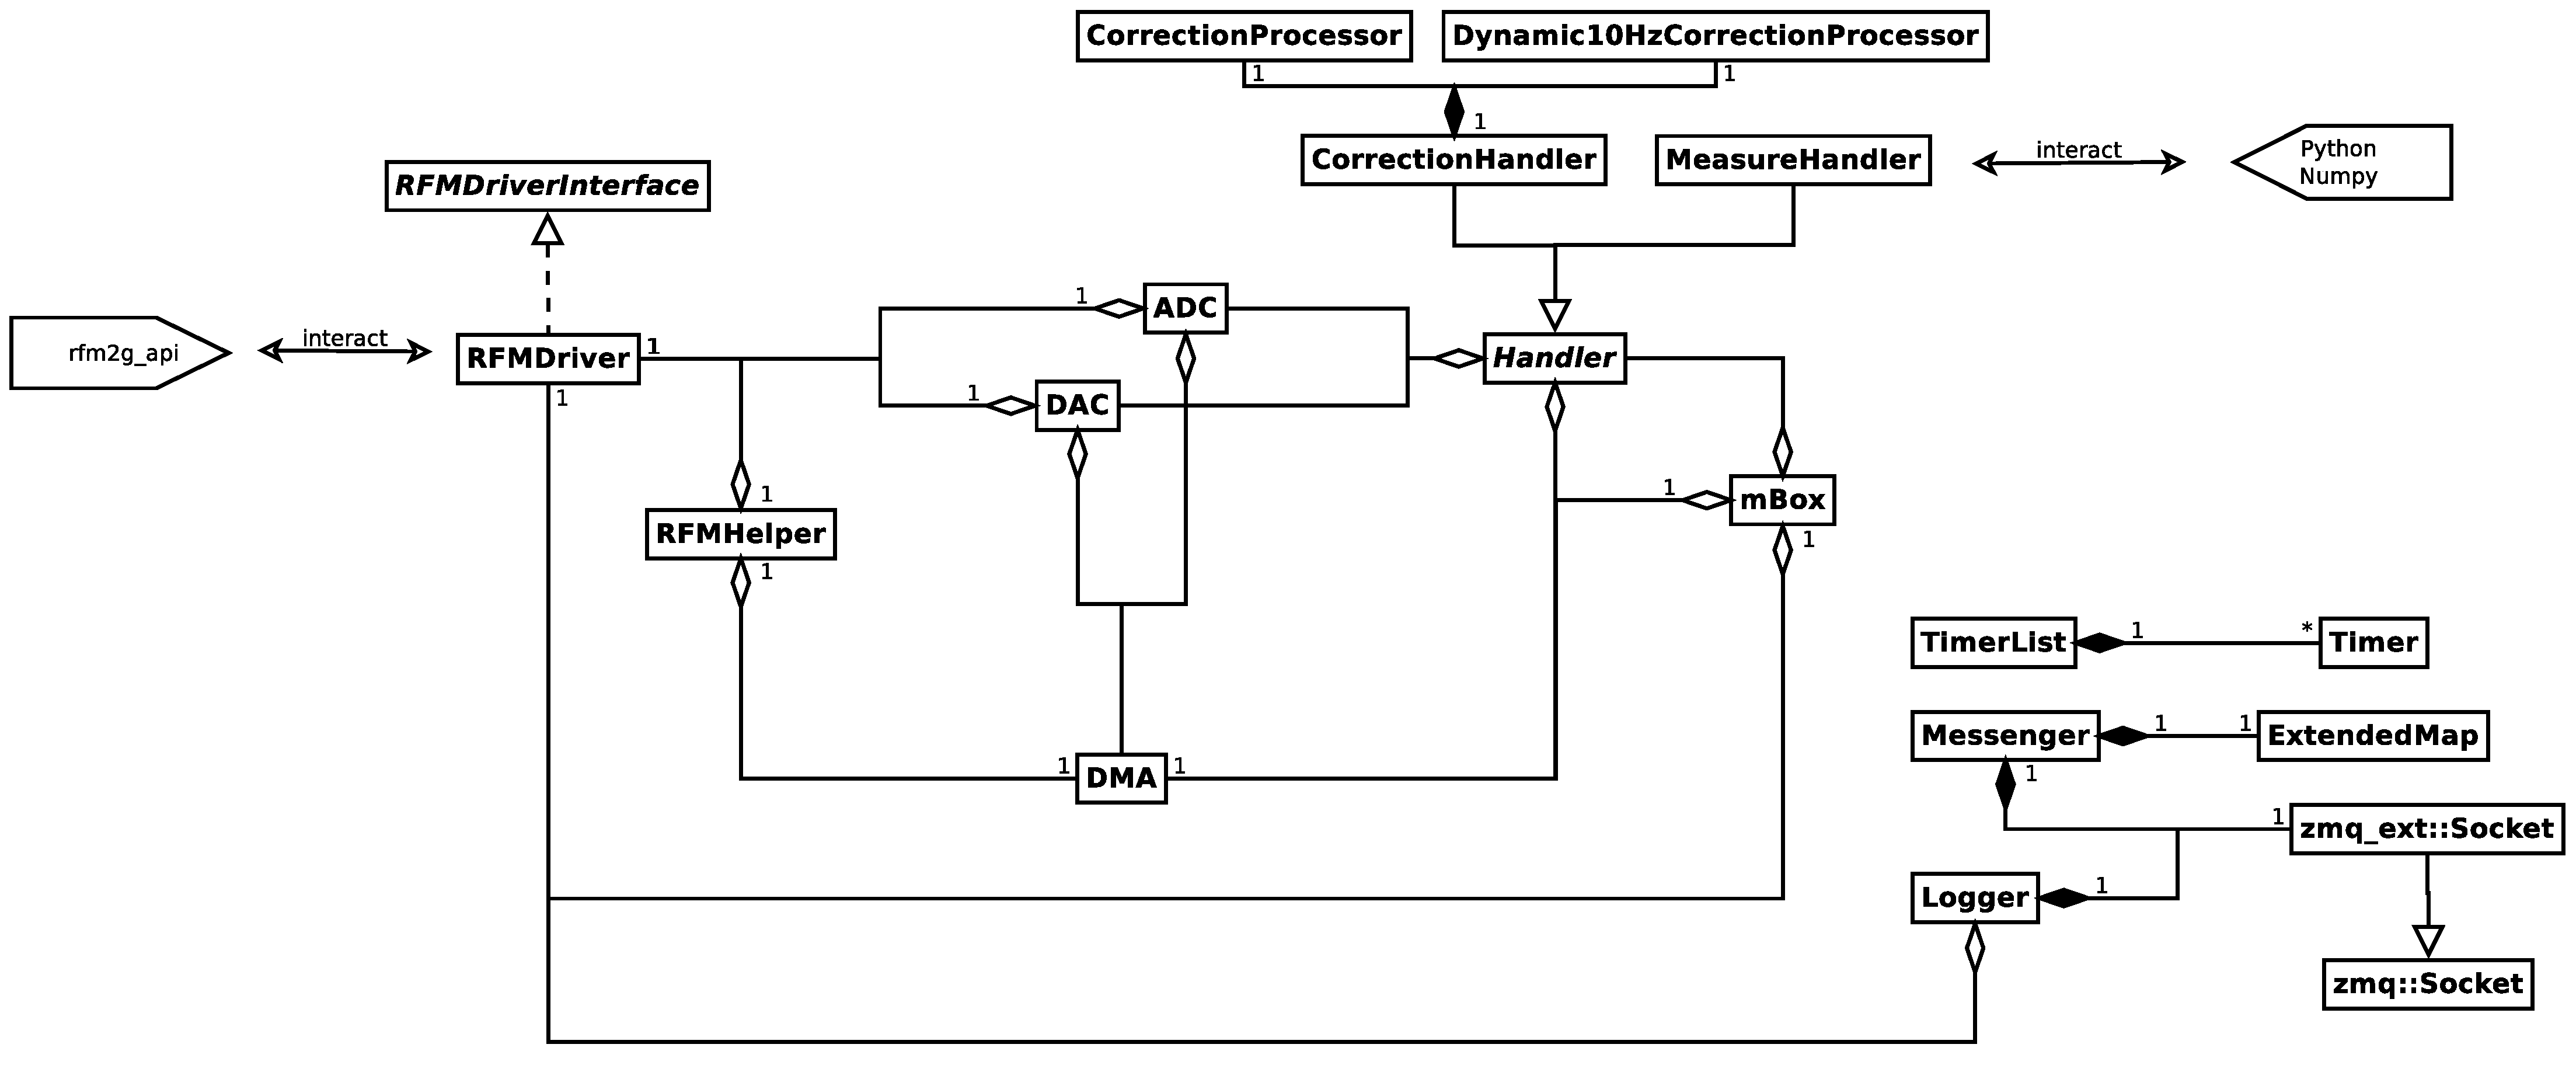
\includegraphics[width=\linewidth]{img/mBox_classDiagram}
    \caption{\label{fig:mbox_class_diag}Class diagram of the mBox++ program}
\end{sidewaysfigure}

The class \texttt{mBox} is the one from which everything begins. It creates the shared objects and deals with the state machine process. It owns a \texttt{Handler} which can be a \texttt{CorrectionHandler} if mBox++ runs in normal mode, or a \texttt{MeasureHandler} if it runs in experiment mode (by default mBox++ runs in correction mode, but it can be started in experiment mode with a python script in input).\todo{les parentheses pourront etre enlevees quand les spec auront ete ecrits}

The actual mathematics (computation of the calculation) happens in the processors. If the handler is a \texttt{CorrectionHandler}, then the processor can be a \texttt{CorrectionProcessor} which does exactly what the \textsc{Matlab} code did (see \cref{sec:correction_state_of_art}) or a \texttt{Dynamic10HzCorrectionProcessor} which implements what was described in \cref{sec:dyn_corr_ex_10Hz}. Else if the handler is a \texttt{MeasureHandler}, the processor is directly the Python script provided by the user.

A handler delegates the actions to objects it owns:
\begin{enumerate}
    \item The \texttt{ADC} reads the data from the ADC reserved area in the RFM.
    \item The handler reads the data from the \texttt{ADC} object, do some conversions (mostly from a integer representation to doubles) and provides the data to its processor that calculates the correction.
    \item The correction is then converted to integers by the handler and provided to the \texttt{DAC} which writes it to the DAC reserved area in the RFM.
\end{enumerate}

To access the RFM, the C functions provided by the constructor are used. An interface \texttt{RFMDriverInterface} is implemented by the \texttt{RFMDriver} which provides a more object oriented version of the C~API.

\remark In order to be able to test the program without having access to a RFM hardware, a second \texttt{RFMDriver} (accessible by compiling with the \texttt{-DDUMMY\_DRIVER=ON} flag) implements the interface: it reads and writes in a 64~Mb binary file that represents the RFM. This can allow to create a simulation of the whole environment and to interact with the program quite easily.

Three modules are statically constructed and globally defined (in their own namespaces):
\begin{itemize}
    \item \texttt{TimerList} which is a "clever" list of \texttt{Timer}s, used to profile the parts of the code. A new or already existing timer can be started with
     \begin{c++}
         TimingModule::addTimer("name_of_timer");           
     \end{c++}
    stopped with 
    \begin{c++}
        TimingModule::timer("name_of_timer").stop();   
    \end{c++}
    and its values shown (in this case once every 1000 times) with
    \begin{c++}
        TimingModule::printAll(Timer::Unit::ms, 1000);
    \end{c++}
    The \texttt{TimimgModule} being global, it can be accessed from everywhere and thus some profiling can be done across objects and functions.

    \item \texttt{Logger} which is a class logging actions and errors. By defaults, errors only are shown to the stdout (standard output stream). Logs and errors are published on a given port (3333 by default) with ZeroMQ and can be read by subscribed services (the logs and errors can thus be output, saved in a file, published on a website stream or whatever crazy idea the user can have). It uses the ZeroMQ Publisher mode. A debug mode is also available (see \texttt{--help} command). It publishes incoming and outgoing values that can be used by other scripts or programs for display, scripting, value-checking... The full description of the uses are given in the Doxygen\footnote{Popular documentation generator that extracts specific comments to produce PDF or HTML documentation. See \url{http://www.stack.nl/~dimitri/doxygen/index.html}} documentation
    
    \item \texttt{Messenger} which is a class for exchanging information with outside scripts and programs. It is listening on a given port (3334 by default). It is using the ZeroMQ Router mode. Every time it receives a request, it processes it and either return the value of the requested variable, or set the given variable to the received value. The difference with the \texttt{Logger} is that the logger publishes values even if no one is listening and sends it when the asked by the code, whereas the \texttt{Messenger} only answers queries. It is notably used in the harmonic correction process described in \cref{sec:dyn_corr_ex_10Hz}: a python script calculates all the phases and amplitudes and sends the outcome, which are then used by \texttt{Dynamic10HzCorrectionProcessor}.
\end{itemize}

\section{Project organization}
The project is organized as followed:
\begin{itemize}
    \item \texttt{/cmake} contains CMake modules to find other libraries and dependencies.
    \item \texttt{/doc} contains resources for the documentation and the generated documentation (which is not synchronized in the version control).
    \item \texttt{/experimentScripts} contains Python scripts that can be used as processor in experiment mode.
    \item \texttt{/python\_tools} contains Python scripts and modules that can be used with the program: the helper for the harmonic correction is there (\texttt{tenHz.py}), a module to communicate with mBox++ through a binary file in dummy mode (\texttt{cbox.py}, \texttt{dummy\_simul.py}) and various helpers to subscribe to the ZeroMQ streams, save data in a specified way...
    \item \texttt{/src} contains all the C++ code to be compiled. Its root contains the core of the project. The rest of the code is split in \texttt{/src/modules}, \texttt{/src/handlers} for a better readability.     
    \end{itemize}
    Finally at the root of the project is \texttt{README.md} file giving the dependencies, how to compile, install and use mBox++. A Doxygen configuration file \texttt{doxygen.conf} let the documentation be generated by starting
    \begin{verbatim}
        doxygen doxygen.conf
    \end{verbatim}
    
\chapter{Search Kick}
Search Kick is called this way because it began as the cleanup and expansion of a \textsc{Matlab} tool conceived by a previous student during his internship. It was originally only able to find kicks in the orbit, in order to localize perturbation sources. It is currently closer to a Python orbit toolbox that allows translating dump data between various formats, localizing perturbations, and other small algorithms for inverting matrices or optimizing signals.


    

\end{document}

